%%%%%%%%%%%%%%%%%%%%%%%%%%%%%%%%%%%%%%%%%%%%%%%%%%%%%%%%%%%%
% File: hw.tex 						   %
% Description: LaTeX template for homework.                %
%
% Feel free to modify it (mainly the 'preamble' file).     %
% Contact hfwei@nju.edu.cn (Hengfeng Wei) for suggestions. %
%%%%%%%%%%%%%%%%%%%%%%%%%%%%%%%%%%%%%%%%%%%%%%%%%%%%%%%%%%%%

%%%%%%%%%%%%%%%%%%%%%%%%%%%%%%%%%%%%%%%%%%%%%%%%%%%%%%%%%%%%%%%%%%%%%%
% IMPORTANT NOTE: Compile this file using 'XeLaTeX' (not 'PDFLaTeX') %
%
% If you are using TeXLive 2016 on windows,                          %
% you may need to check the following post:                          %
% https://tex.stackexchange.com/q/325278/23098                       %
%%%%%%%%%%%%%%%%%%%%%%%%%%%%%%%%%%%%%%%%%%%%%%%%%%%%%%%%%%%%%%%%%%%%%%

\documentclass[11pt, a4paper, UTF8]{ctexart}
%%%%%%%%%%%%%%%%%%%%%%%%%%%%%%%%%%%
% File: preamble.tex
%%%%%%%%%%%%%%%%%%%%%%%%%%%%%%%%%%%

\usepackage[top = 1.5cm]{geometry}

% Set fonts commands
\newcommand{\song}{\CJKfamily{song}} 
\newcommand{\hei}{\CJKfamily{hei}} 
\newcommand{\kai}{\CJKfamily{kai}} 
\newcommand{\fs}{\CJKfamily{fs}}

\newcommand{\me}[2]{\author{{\bfseries 姓名:}\underline{#1}\hspace{2em}{\bfseries 学号:}\underline{#2}}}

% Always keep this.
\newcommand{\noplagiarism}{
  \begin{center}
    \fbox{\begin{tabular}{@{}c@{}}
      请独立完成作业,不得抄袭。\\
      若参考了其它资料,请给出引用。\\
      鼓励讨论,但需独立书写解题过程。
    \end{tabular}}
  \end{center}
}

% Each hw consists of three parts:
% (1) this homework
\newcommand{\beginthishw}{\part{作业}}
% (2) corrections (Optional)
\newcommand{\begincorrection}{\part{订正}}
% (3) any feedback (Optional)
\newcommand{\beginfb}{\part{反馈}}

% For math
\usepackage{amsmath}
\usepackage{amsfonts}
\usepackage{amssymb}

% Define theorem-like environments
\usepackage[amsmath, thmmarks]{ntheorem}

\theoremstyle{break}
\theorembodyfont{\song}
\theoremseparator{}
\newtheorem*{problem}{题目}

\theorempreskip{2.0\topsep}
\theoremheaderfont{\kai\bfseries}
\theoremseparator{:}
% \newtheorem*{remark}{注}
\theorempostwork{\bigskip\hrule}
\newtheorem*{solution}{解答}
\theorempostwork{\bigskip\hrule}
\newtheorem*{revision}{订正}

\theoremstyle{plain}
\newtheorem*{cause}{错因分析}
\newtheorem*{remark}{注}

\theoremstyle{break}
\theorempostwork{\bigskip\hrule}
\theoremsymbol{\ensuremath{\Box}}
\newtheorem*{proof}{证明}

\renewcommand\figurename{图}
\renewcommand\tablename{表}

% For figures
% for fig with caption: #1: width/size; #2: fig file; #3: fig caption
\newcommand{\fig}[3]{
  \begin{figure}[htp]
    \centering
      \includegraphics[#1]{#2}
      \caption{#3}
  \end{figure}
}

% for fig without caption: #1: width/size; #2: fig file
\newcommand{\fignocaption}[2]{
  \begin{figure}[htp]
    \centering
    \includegraphics[#1]{#2}
  \end{figure}
}  % modify this file if necessary
\usepackage{graphicx}
\usepackage{url}
\usepackage{float}

%%%%%%%%%%%%%%%%%%%%
\title{第三次作业:边缘检测和边缘连接}
\me{丁保荣}{171860509}
\date{\today}     % you can specify a date like ``2017年9月30日''.
%%%%%%%%%%%%%%%%%%%%
\begin{document}

\maketitle


\tableofcontents
\newpage
%%%%%%%%%%%%%%%%%%%%

\section{边缘检测}

对于边缘检测,我一共实现了四种算法:基于sobel算子的边缘检测器、基于prewitt算子的边缘检测器、Marr-Hildreth边缘检测器、Canny边缘检测器。

\subsection{基于sobel算子的边缘检测器}

\subsubsection{实现原理}
基于sobel算子的边缘检测器的实现在$sobel.m$文件中,主要的过程是
\begin{enumerate}
  \item 先对原图像$G$进行高斯滤波得到$G'$ (主要是为了减小噪声的影响)
  \item 对$G'$进行$X$方向的sobel滤波,得到$G_X'$
  \item 对$G'$进行$Y$方向的sobel滤波,得到$G_Y'$
  \item 将$X$方向和$Y$方向的滤波结果进行叠加。得到$new_G$
  \item 根据阈值,对$new_G$进行二值化,得到输出图像
\end{enumerate}
其中第1步中的高斯滤波可以根据图像有无噪声进行选择,如果图像没有噪声,可以选择不进行高斯滤波。

\subsubsection{实现效果}


\begin{figure}[H]
  \centering
  \begin{minipage}[t]{0.48\textwidth}
  \centering
  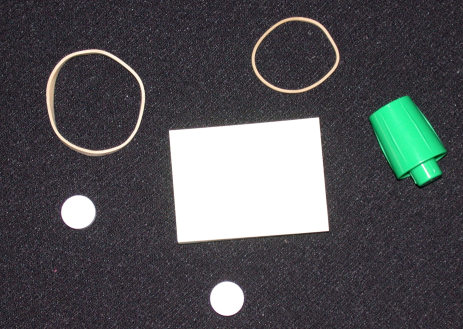
\includegraphics[width=7cm]{rubberband_cap.png}
  \caption{原图}
  \end{minipage}
  \begin{minipage}[t]{0.48\textwidth}
  \centering
  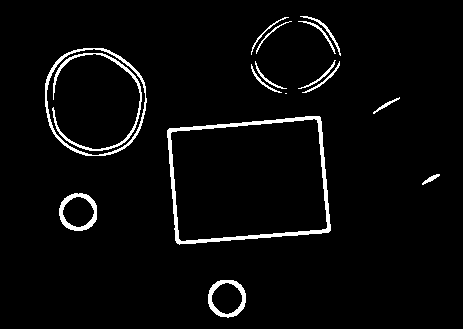
\includegraphics[width=7cm]{sobel_all_rubberband_cap.png}
  \caption{sobel滤波后的}
  \end{minipage}
\end{figure}



\begin{figure}[H]
  \centering
  \begin{minipage}[t]{0.48\textwidth}
  \centering
  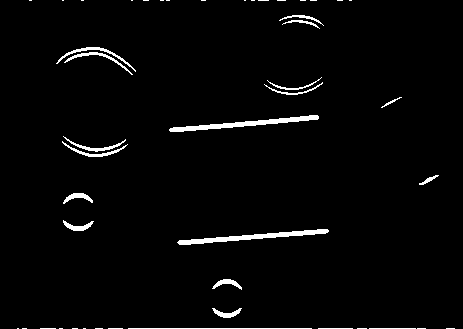
\includegraphics[width=7cm]{sobel_X_rubberband_cap.png}
  \caption{只进行X方向滤波}
  \end{minipage}
  \begin{minipage}[t]{0.48\textwidth}
  \centering
  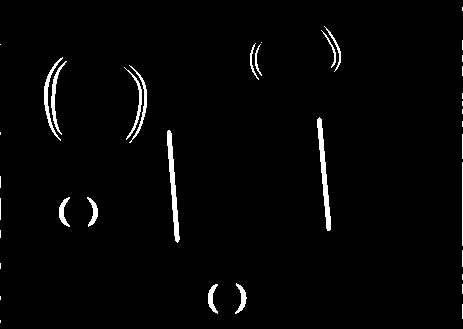
\includegraphics[width=7cm]{sobel_Y_rubberband_cap.png}
  \caption{只进行Y方向滤波}
  \end{minipage}
\end{figure}

如果只进行$X$方向或$Y$方向的滤波,会发现只有一个方向的边缘比较明显,另一个方向的边缘并不是很明显。



下面是其他一些图像经过sobel滤波后的结果:


\begin{figure}[H]
  \centering
  \begin{minipage}[t]{0.48\textwidth}
  \centering
  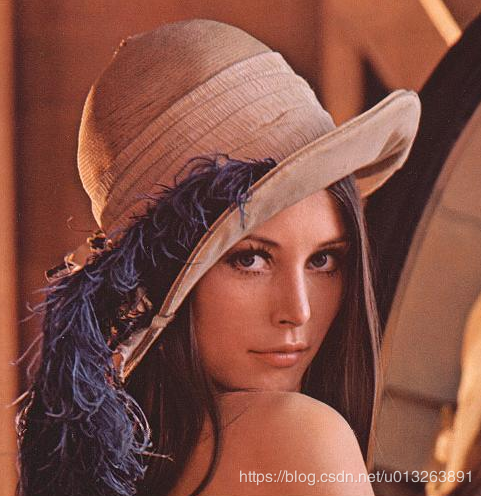
\includegraphics[width=7cm]{lena.png}
  \caption{原图}
  \end{minipage}
  \begin{minipage}[t]{0.48\textwidth}
  \centering
  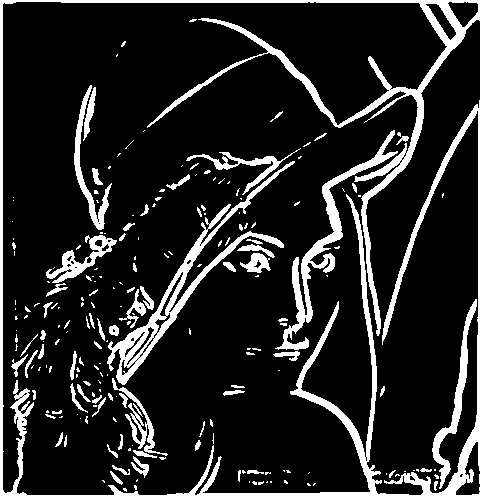
\includegraphics[width=7cm]{sobel_all_lena.png}
  \caption{sobel滤波后的}
  \end{minipage}
\end{figure}


\begin{figure}[H]
  \centering
  \begin{minipage}[t]{0.48\textwidth}
  \centering
  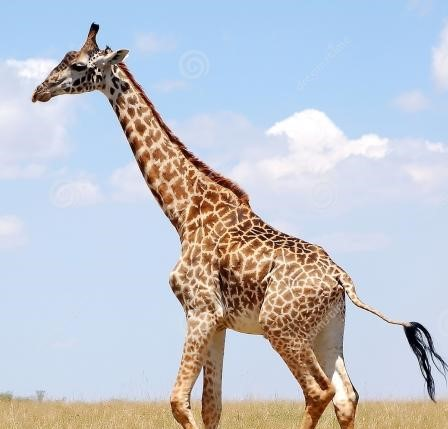
\includegraphics[width=7cm]{giraffe.jpg}
  \caption{原图}
  \end{minipage}
  \begin{minipage}[t]{0.48\textwidth}
  \centering
  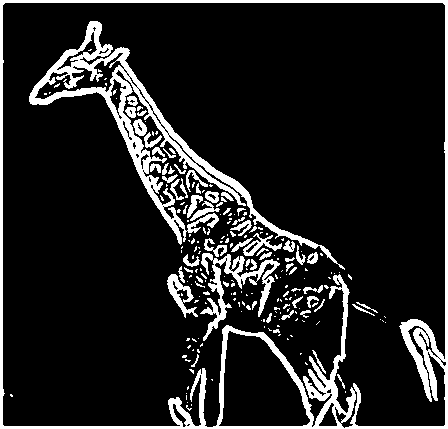
\includegraphics[width=7cm]{sobel_all_giraffe.png}
  \caption{sobel滤波后的}
  \end{minipage}
\end{figure}

\begin{figure}[H]
  \centering
  \begin{minipage}[t]{0.48\textwidth}
  \centering
  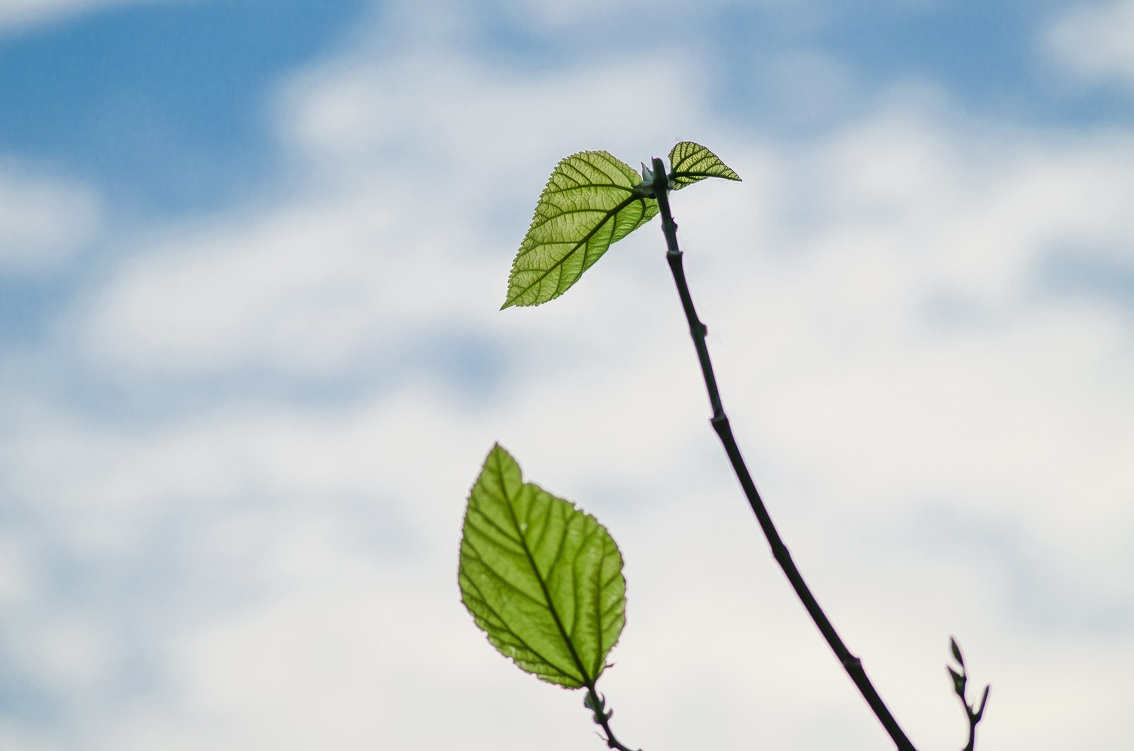
\includegraphics[width=7cm]{leaf.jpg}
  \caption{原图}
  \end{minipage}
  \begin{minipage}[t]{0.48\textwidth}
  \centering
  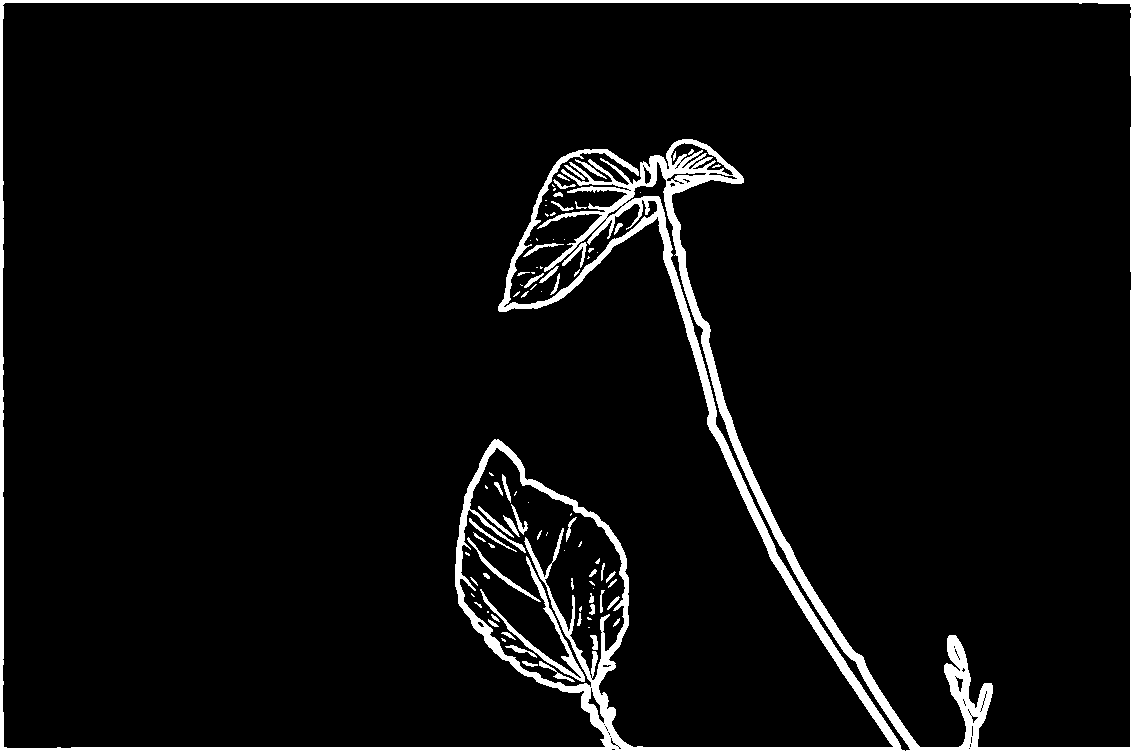
\includegraphics[width=7cm]{sobel_all_leaf.png}
  \caption{sobel滤波后的}
  \end{minipage}
\end{figure}


\begin{figure}[H]
  \centering
  \begin{minipage}[t]{0.48\textwidth}
  \centering
  
\includegraphics[width=7cm]{ayu.jpg}
  \caption{原图}
  \end{minipage}
  \begin{minipage}[t]{0.48\textwidth}
  \centering
  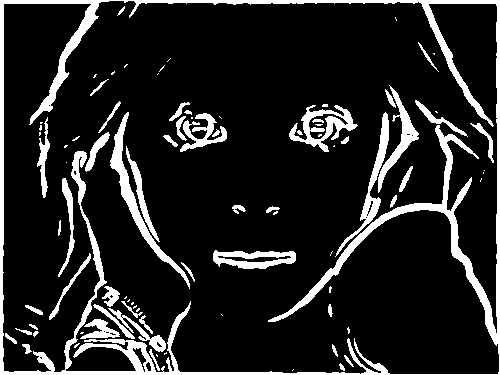
\includegraphics[width=7cm]{sobel_all_ayu.png}
  \caption{sobel滤波后的}
  \end{minipage}
\end{figure}


\begin{figure}[H]
  \centering
  \begin{minipage}[t]{0.48\textwidth}
  \centering
  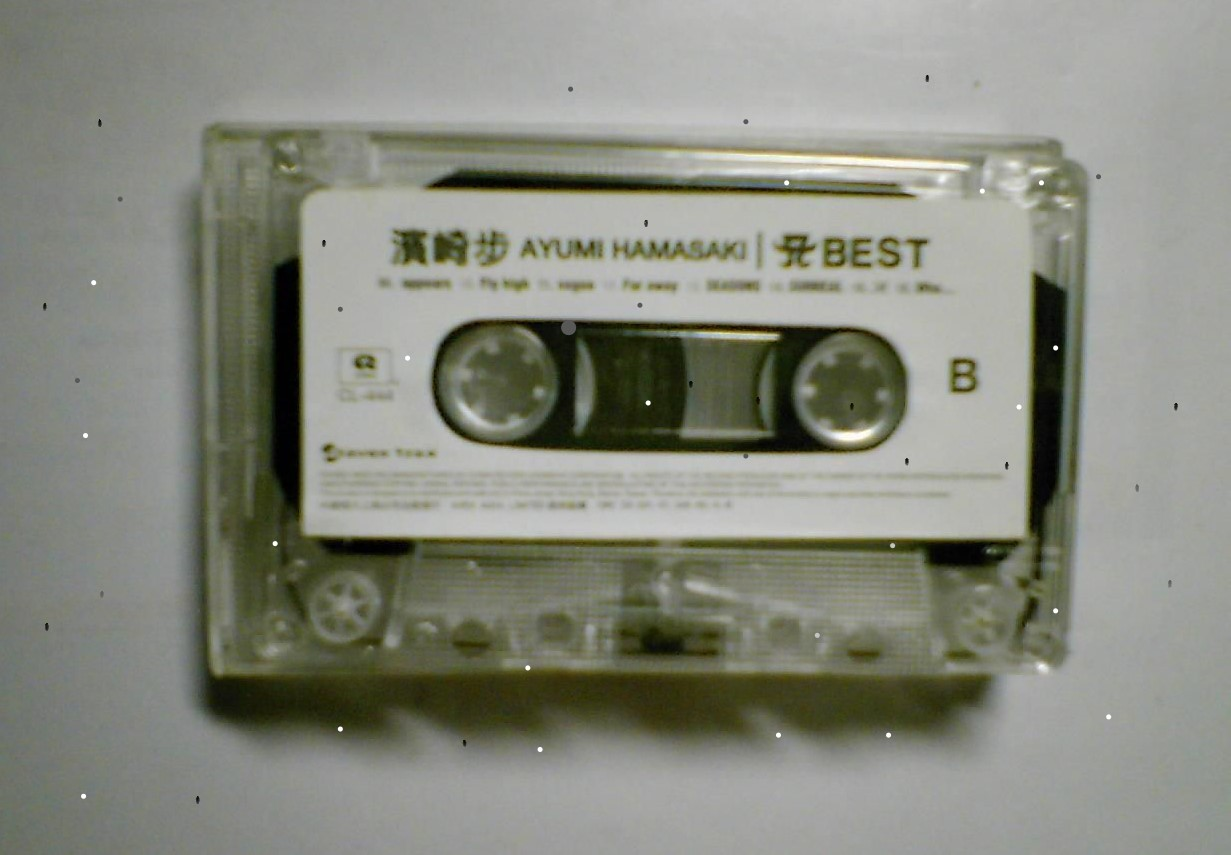
\includegraphics[width=7cm]{noise.jpg}
  \caption{原图}
  \end{minipage}
  \begin{minipage}[t]{0.48\textwidth}
  \centering
  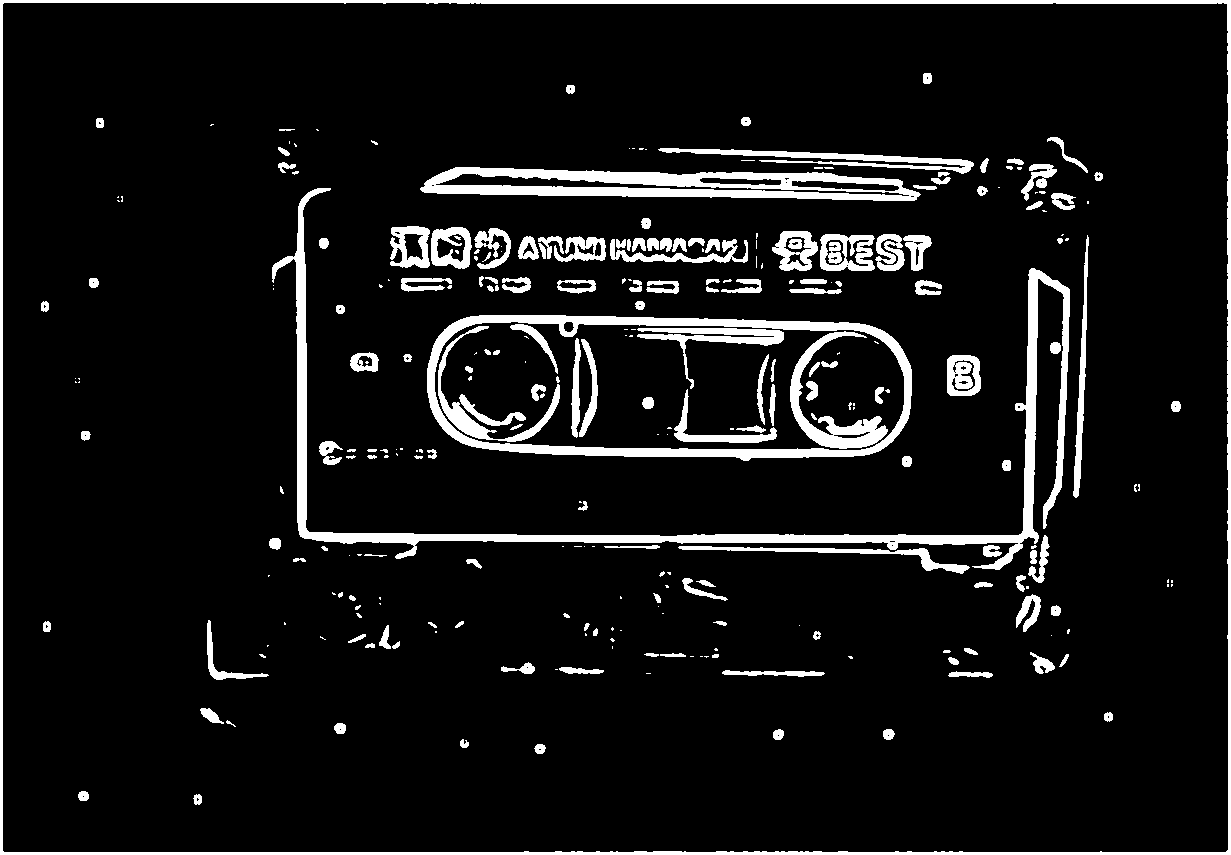
\includegraphics[width=7cm]{sobel_all_noise.png}
  \caption{sobel滤波后的}
  \end{minipage}
\end{figure}



\subsection{基于prewitt算子的边缘检测器}

\subsubsection{实现原理}
基于prewitt算子的边缘检测器的实现在$prewitt.m$文件中,实现方法与sobel算子类似,主要的过程是
\begin{enumerate}
  \item 先对原图像$G$进行高斯滤波得到$G'$ (主要是为了减小噪声的影响)
  \item 对$G'$进行$X$方向的prewitt滤波,得到$G_X'$
  \item 对$G'$进行$Y$方向的prewitt滤波,得到$G_Y'$
  \item 将$X$方向和$Y$方向的滤波结果进行叠加。得到$new_G$
  \item 根据阈值,对$new_G$进行二值化,得到输出图像
\end{enumerate}
其中第1步中的高斯滤波可以根据图像有无噪声进行选择,如果图像没有噪声,可以选择不进行高斯滤波。

\subsubsection{实现效果}

\begin{figure}[H]
  \centering
  \begin{minipage}[t]{0.48\textwidth}
  \centering
  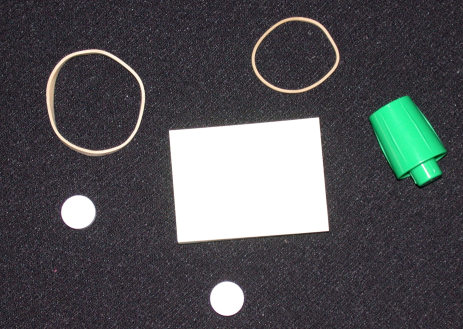
\includegraphics[width=7cm]{rubberband_cap.png}
  \caption{原图}
  \end{minipage}
  \begin{minipage}[t]{0.48\textwidth}
  \centering
  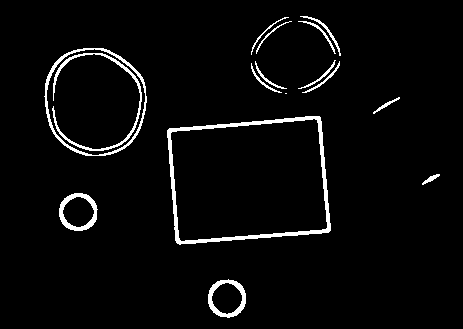
\includegraphics[width=7cm]{prewitt_all_rubberband_cap.png}
  \caption{prewitt滤波后的}
  \end{minipage}
\end{figure}



\begin{figure}[H]
  \centering
  \begin{minipage}[t]{0.48\textwidth}
  \centering
  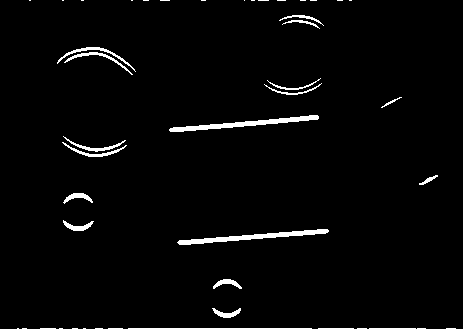
\includegraphics[width=7cm]{prewitt_X_rubberband_cap.png}
  \caption{只进行X方向滤波}
  \end{minipage}
  \begin{minipage}[t]{0.48\textwidth}
  \centering
  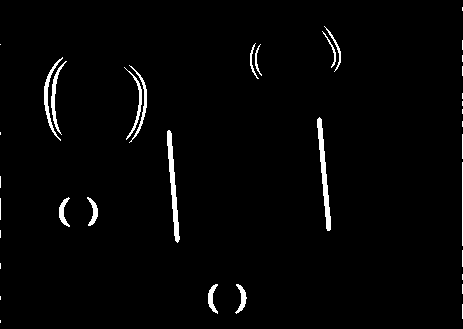
\includegraphics[width=7cm]{prewitt_Y_rubberband_cap.png}
  \caption{只进行Y方向滤波}
  \end{minipage}
\end{figure}

与sobel算子类似,如果只进行$X$方向或$Y$方向的滤波,会发现只有一个方向的边缘比较明显,另一个方向的边缘并不是很明显。



下面是其他一些图像经过prewitt滤波后的结果:


\begin{figure}[H]
  \centering
  \begin{minipage}[t]{0.48\textwidth}
  \centering
  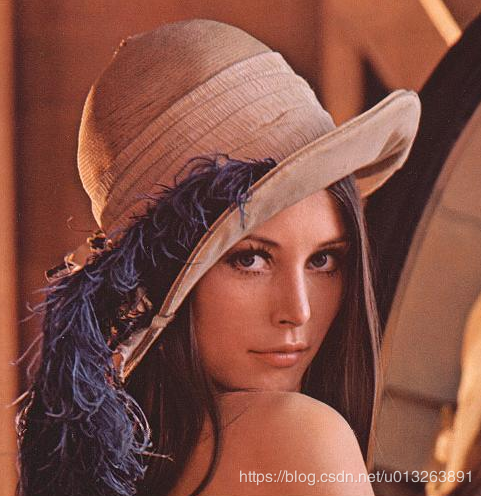
\includegraphics[width=7cm]{lena.png}
  \caption{原图}
  \end{minipage}
  \begin{minipage}[t]{0.48\textwidth}
  \centering
  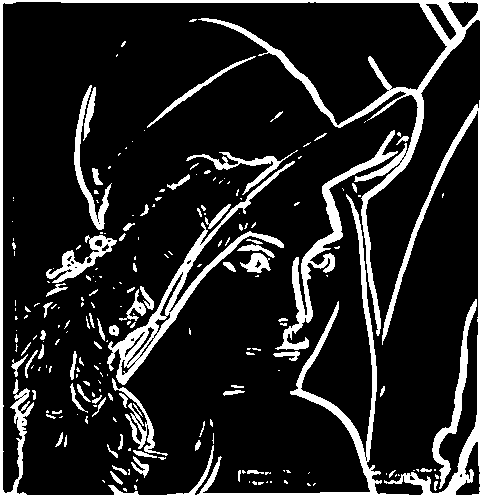
\includegraphics[width=7cm]{prewitt_all_lena.png}
  \caption{prewitt滤波后的}
  \end{minipage}
\end{figure}


\begin{figure}[H]
  \centering
  \begin{minipage}[t]{0.48\textwidth}
  \centering
  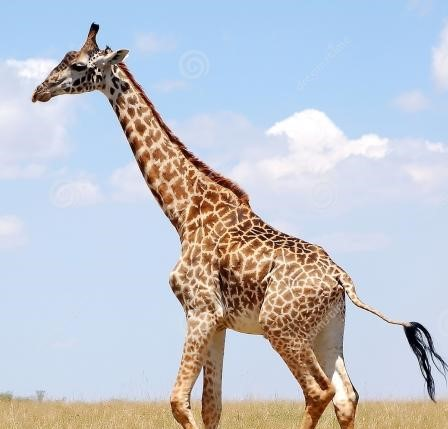
\includegraphics[width=7cm]{giraffe.jpg}
  \caption{原图}
  \end{minipage}
  \begin{minipage}[t]{0.48\textwidth}
  \centering
  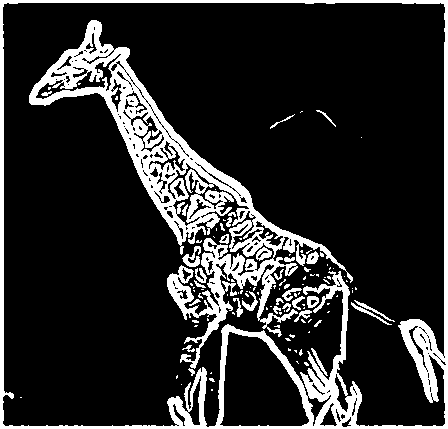
\includegraphics[width=7cm]{prewitt_all_giraffe.png}
  \caption{prewitt滤波后的}
  \end{minipage}
\end{figure}

\begin{figure}[H]
  \centering
  \begin{minipage}[t]{0.48\textwidth}
  \centering
  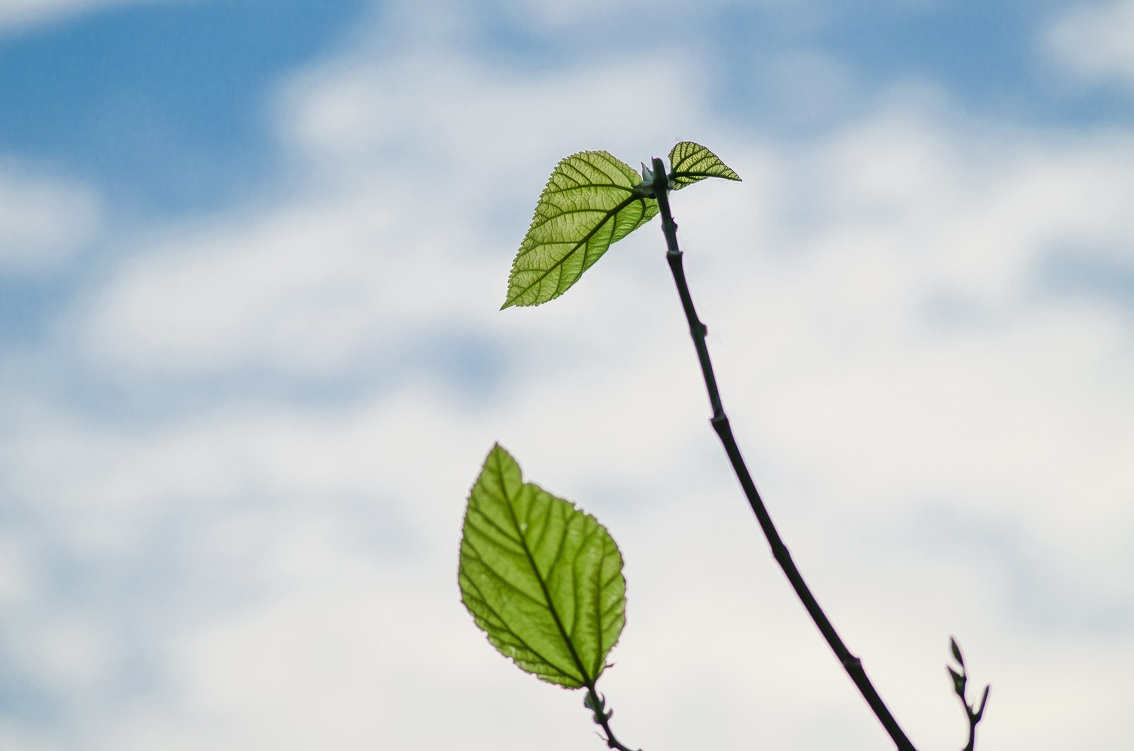
\includegraphics[width=7cm]{leaf.jpg}
  \caption{原图}
  \end{minipage}
  \begin{minipage}[t]{0.48\textwidth}
  \centering
  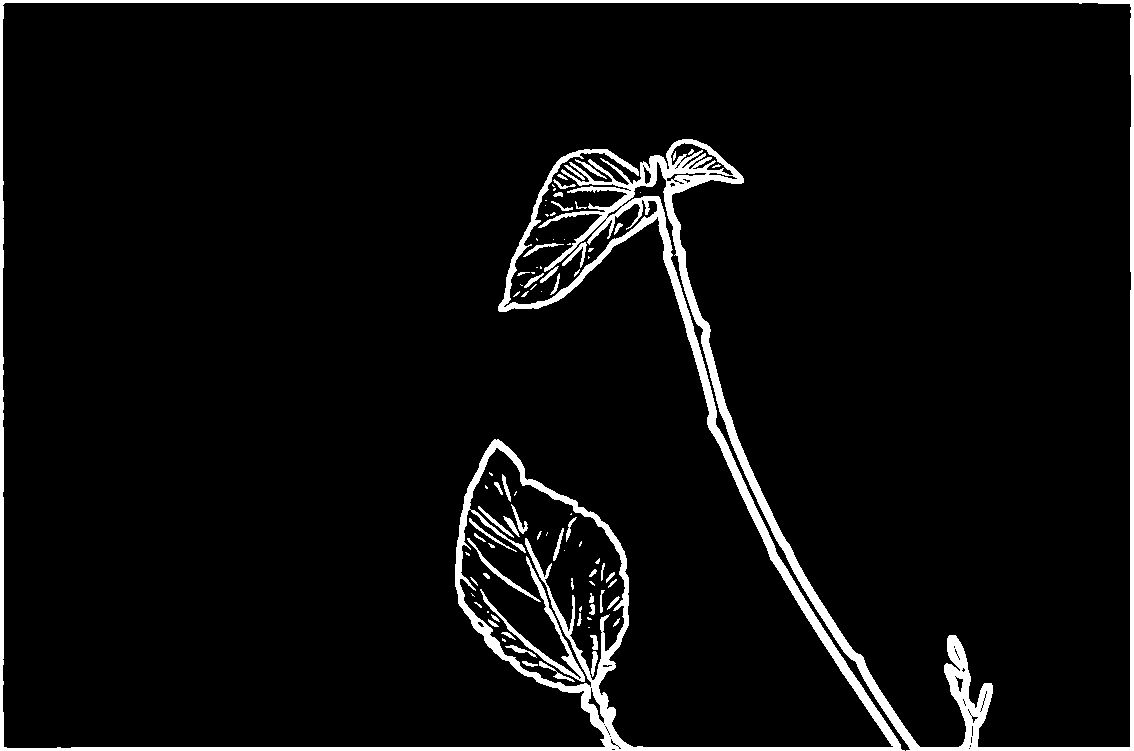
\includegraphics[width=7cm]{prewitt_all_leaf.png}
  \caption{prewitt滤波后的}
  \end{minipage}
\end{figure}


\begin{figure}[H]
  \centering
  \begin{minipage}[t]{0.48\textwidth}
  \centering
  
\includegraphics[width=7cm]{ayu.jpg}
  \caption{原图}
  \end{minipage}
  \begin{minipage}[t]{0.48\textwidth}
  \centering
  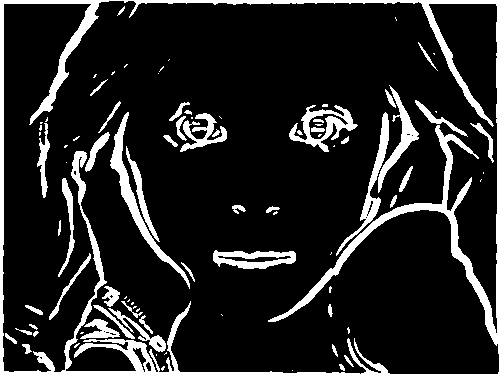
\includegraphics[width=7cm]{prewitt_all_ayu.png}
  \caption{prewitt滤波后的}
  \end{minipage}
\end{figure}

\begin{figure}[H]
  \centering
  \begin{minipage}[t]{0.48\textwidth}
  \centering
  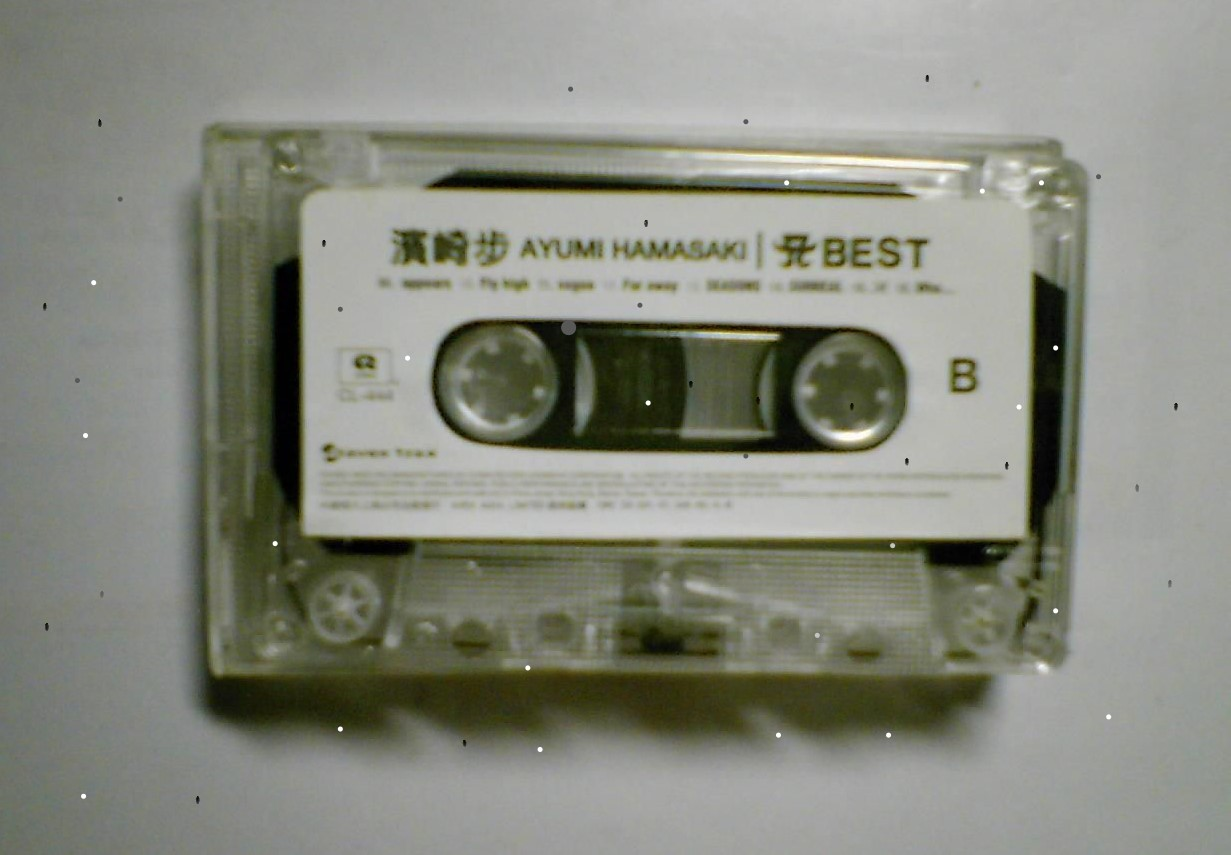
\includegraphics[width=7cm]{noise.jpg}
  \caption{原图}
  \end{minipage}
  \begin{minipage}[t]{0.48\textwidth}
  \centering
  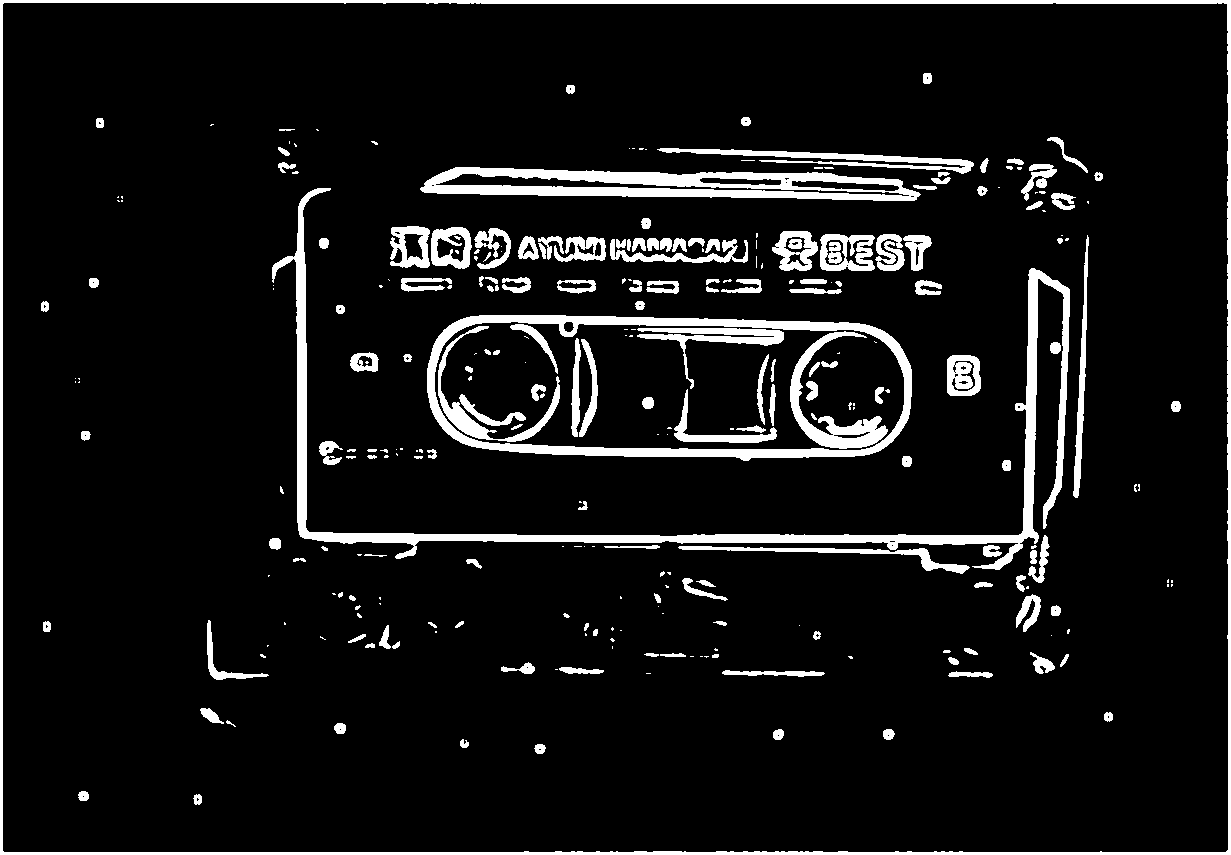
\includegraphics[width=7cm]{prewitt_all_noise.png}
  \caption{prewitt滤波后的}
  \end{minipage}
\end{figure}

\subsection{prewitt算子和sobel算子的比较}

$X$方向的prewitt算子:$$
  \begin{bmatrix}
    1 & 1 & 1 \\
    0 & 0 & 0 \\
    -1 & -1 & -1 
  \end{bmatrix} $$

  $X$方向的sobel算子: $$
  \begin{bmatrix}
    1 & 2 & 1 \\
    0 & 0 & 0 \\
    -1 & -2 & -1 
  \end{bmatrix} $$

    在矩阵表示上,我们发现sobel算子和prewitt算子的差异很小,所以我们看他们效果也差不多。因为没有非最大抑制,所以sobel算子和prewitt算子产生的图像边缘都比较粗

    \begin{figure}[H]
      \centering
      \begin{minipage}[t]{0.48\textwidth}
      \centering
      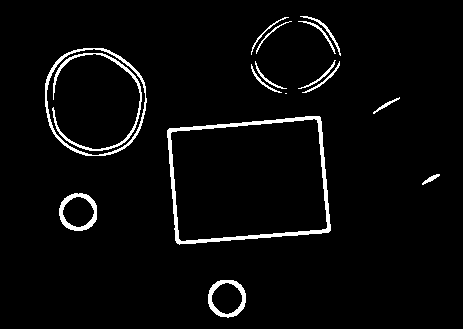
\includegraphics[width=7cm]{sobel_all_rubberband_cap.png}
      \caption{sobel滤波后的}
      \end{minipage}
      \begin{minipage}[t]{0.48\textwidth}
      \centering
      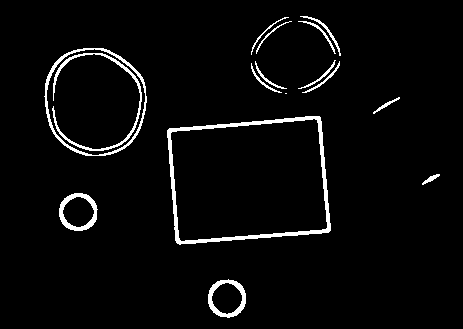
\includegraphics[width=7cm]{prewitt_all_rubberband_cap.png}
      \caption{prewitt滤波后的}
      \end{minipage}
    \end{figure}

    \begin{figure}[H]
      \centering
      \begin{minipage}[t]{0.48\textwidth}
      \centering
      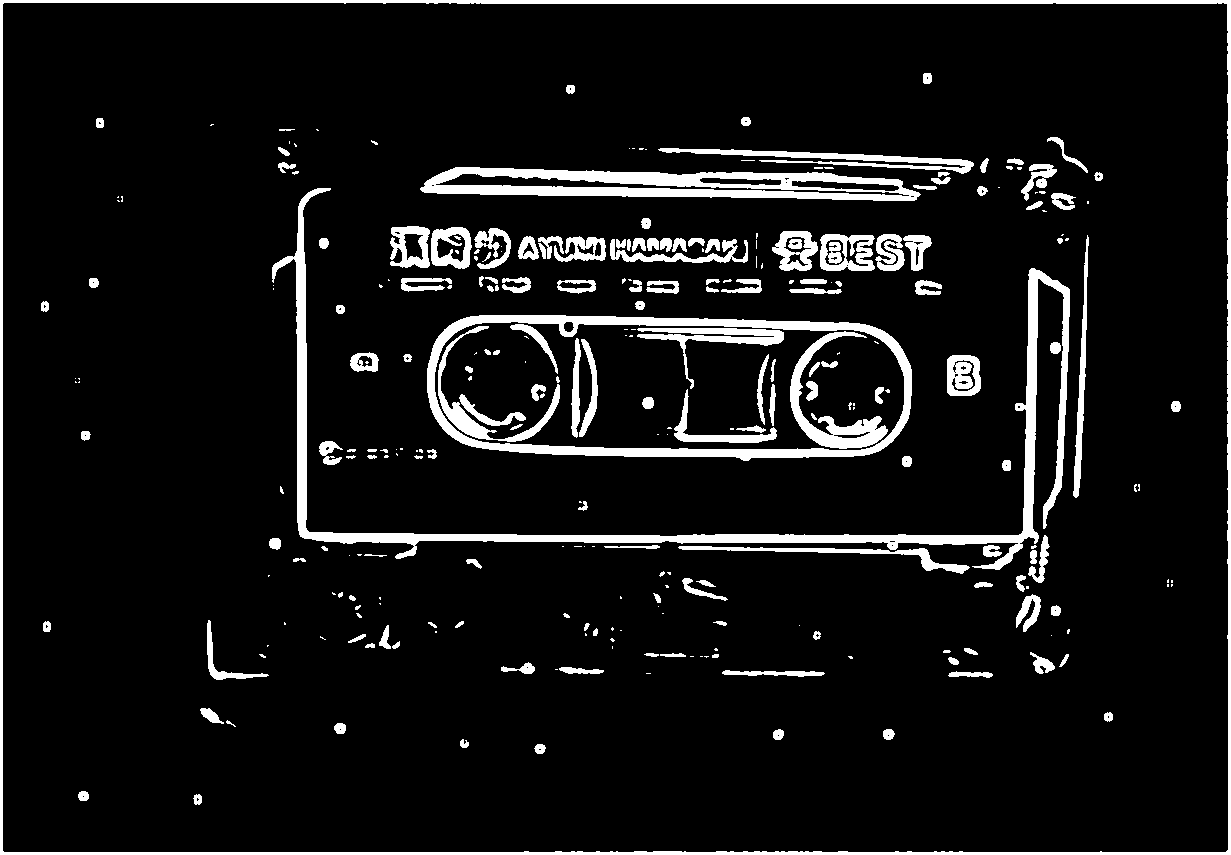
\includegraphics[width=7cm]{sobel_all_noise.png}
      \caption{sobel滤波后的}
      \end{minipage}
      \begin{minipage}[t]{0.48\textwidth}
      \centering
      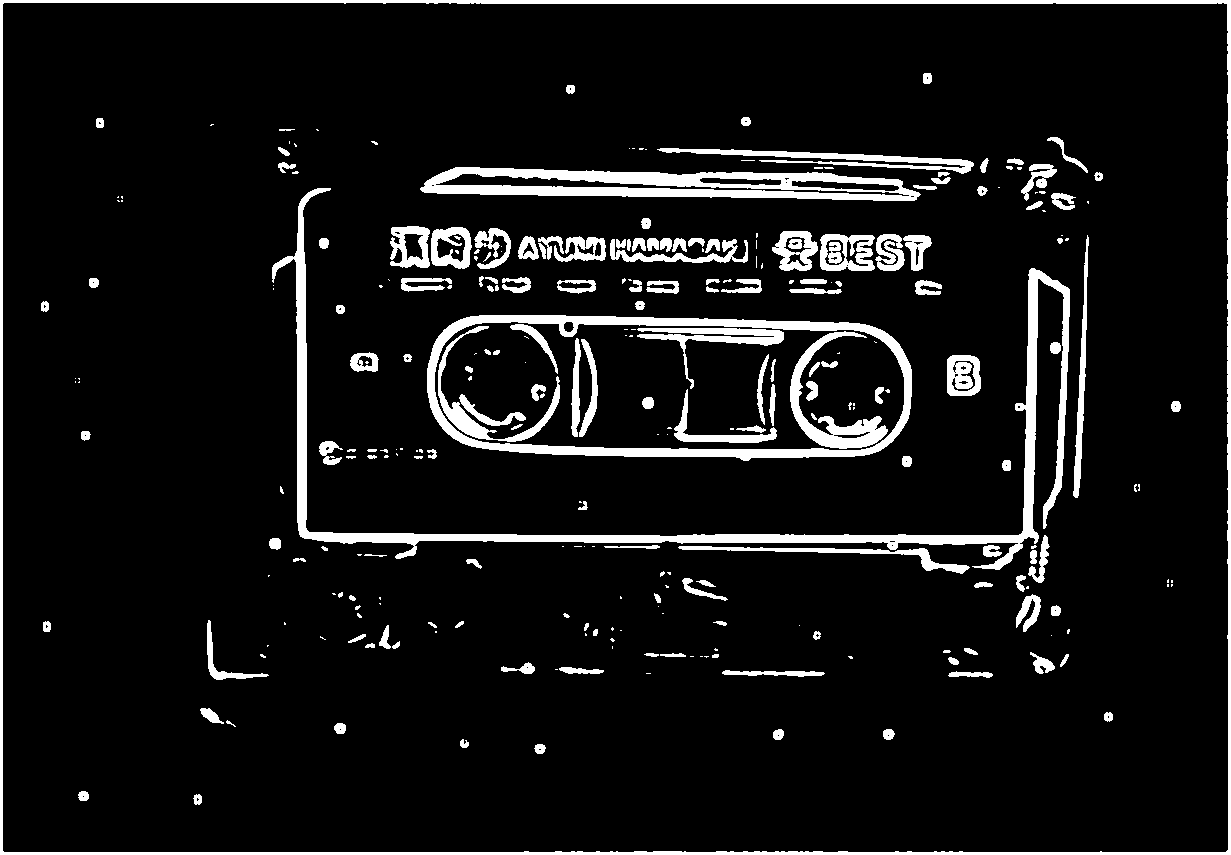
\includegraphics[width=7cm]{prewitt_all_noise.png}
      \caption{prewitt滤波后的}
      \end{minipage}
    \end{figure}


\subsection{Marr-Hildreth边缘检测器}

\subsubsection{实现原理}
Marr-Hildreth边缘检测器的实现在$MarrHildreth.m$文件中,实现方法与sobel算子类似,主要的过程是
 \begin{enumerate}
   \item 用$n \times n$的高斯低通滤波器平滑图像$G$得到$G'$($n$是大于等于$6\sigma$的最小奇数)
   \item 计算$G'$的拉普拉斯$G_L'$
   \item 寻找$G_L'$的零交叉(任意方向的两个邻居符号相反且差值大于一定的阈值)
 \end{enumerate}
Marr-Hildreth主要需要设置的参数有$n$、阈值系数($th$),都和输入图像有一定的关系。其中我对不同图像设置不同的阈值系数($th$)以达到最好的效果。如果阈值比例设置得太低,会有很多噪点,但阈值比例设置得太高,又可能会使得边缘断开。

\subsubsection{实现效果}

\begin{figure}[H]
  \centering
  \begin{minipage}[t]{0.48\textwidth}
  \centering
  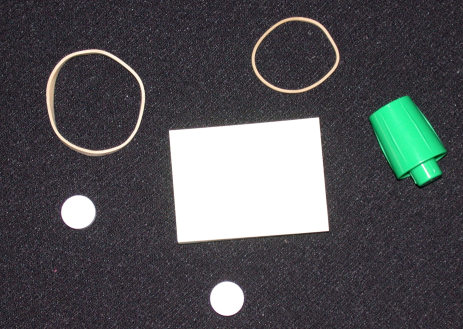
\includegraphics[width=7cm]{rubberband_cap.png}
  \caption{原图}
  \end{minipage}
  \begin{minipage}[t]{0.48\textwidth}
  \centering
  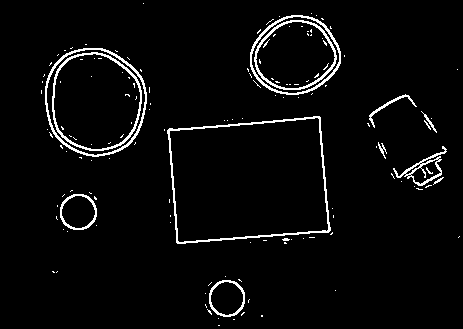
\includegraphics[width=7cm]{MH_alpha=0.35_rubberband_cap.png}
  \caption{MH处理后的($th=0.35$)}
  \end{minipage}
\end{figure}

我发现设置不同阈值系数对于图像的效果影响还是很大的:如下面两张图的阈值比例就设置得不太好。

\begin{figure}[H]
  \centering
  \begin{minipage}[t]{0.48\textwidth}
  \centering
  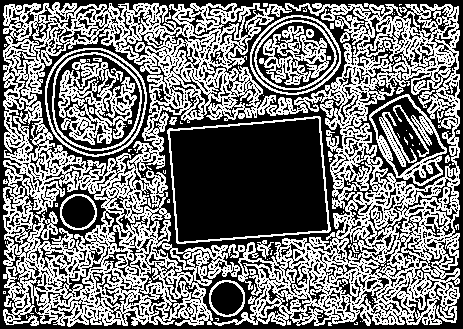
\includegraphics[width=7cm]{MH_alpha=0.04_rubberband_cap.png}
  \caption{MH处理后的($th=0.04$)}
  \end{minipage}
  \begin{minipage}[t]{0.48\textwidth}
  \centering
  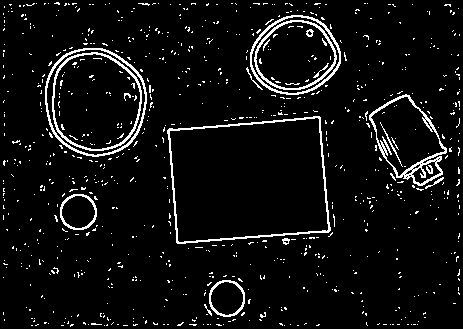
\includegraphics[width=7cm]{MH_alpha=0.2_rubberband_cap.png}
  \caption{MH处理后的($th=0.2$)}
  \end{minipage}
\end{figure}


下面展示一下其他图片用Marr-Hildreth边缘检测器的效果:
\begin{figure}[H]
  \centering
  \begin{minipage}[t]{0.48\textwidth}
  \centering
  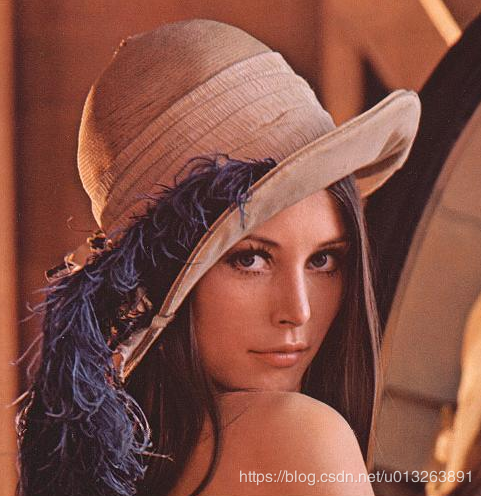
\includegraphics[width=7cm]{lena.png}
  \caption{原图}
  \end{minipage}
  \begin{minipage}[t]{0.48\textwidth}
  \centering
  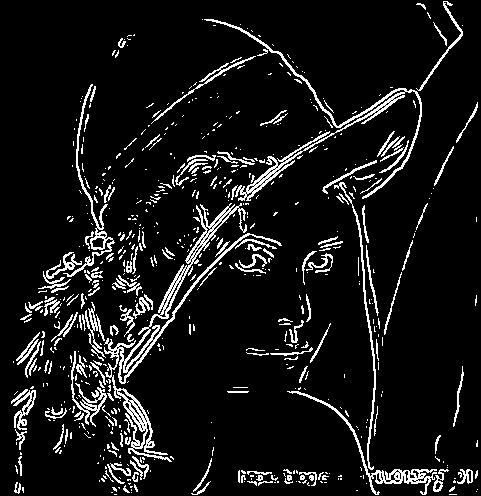
\includegraphics[width=7cm]{MH_alpha=0.3_lena.png}
  \caption{MH处理后的($th=0.3$)}
  \end{minipage}
\end{figure}


\begin{figure}[H]
  \centering
  \begin{minipage}[t]{0.48\textwidth}
  \centering
  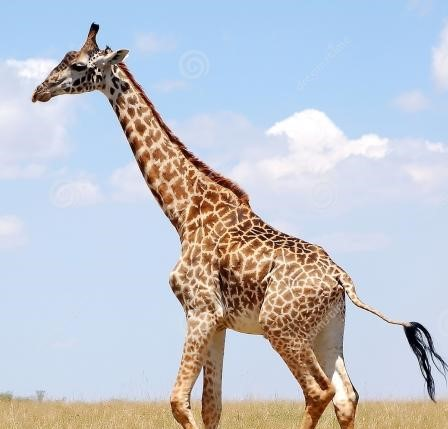
\includegraphics[width=7cm]{giraffe.jpg}
  \caption{原图}
  \end{minipage}
  \begin{minipage}[t]{0.48\textwidth}
  \centering
  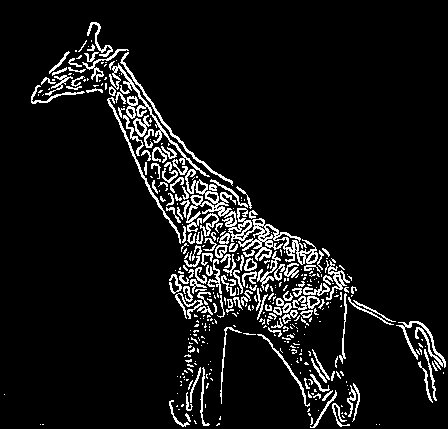
\includegraphics[width=7cm]{MH_alpha=0.35_giraffe.png}
  \caption{MH处理后的($th=0.35$)}
  \end{minipage}
\end{figure}

\begin{figure}[H]
  \centering
  \begin{minipage}[t]{0.48\textwidth}
  \centering
  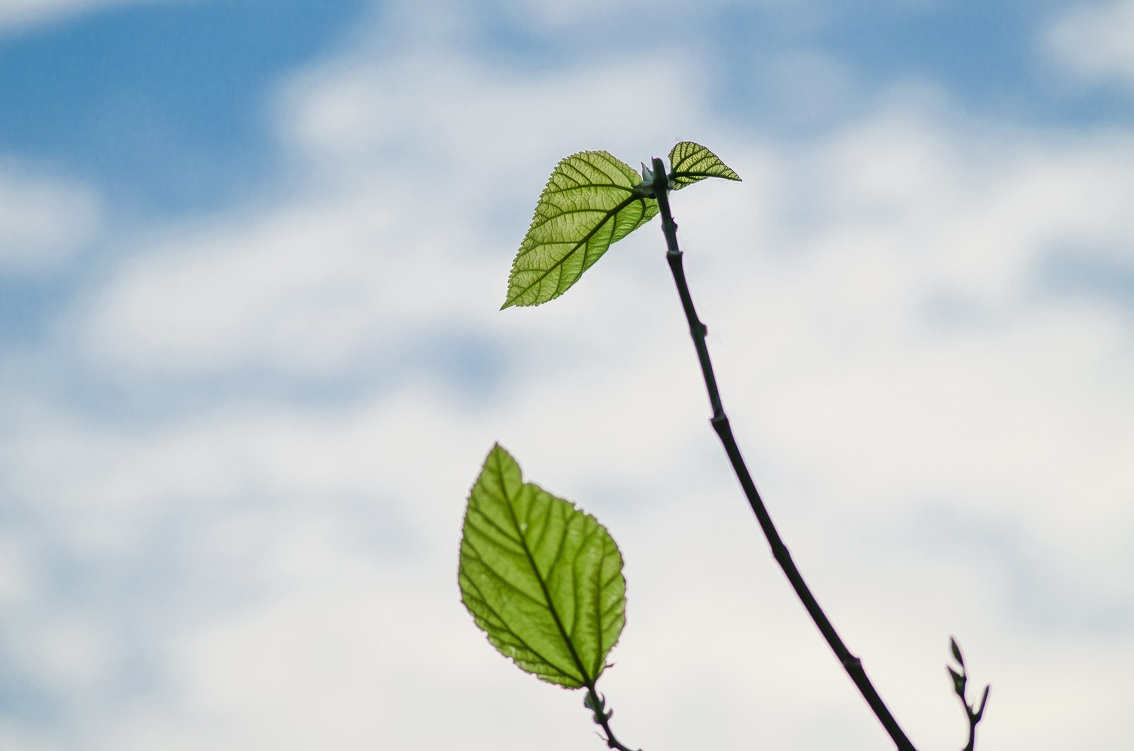
\includegraphics[width=7cm]{leaf.jpg}
  \caption{原图}
  \end{minipage}
  \begin{minipage}[t]{0.48\textwidth}
  \centering
  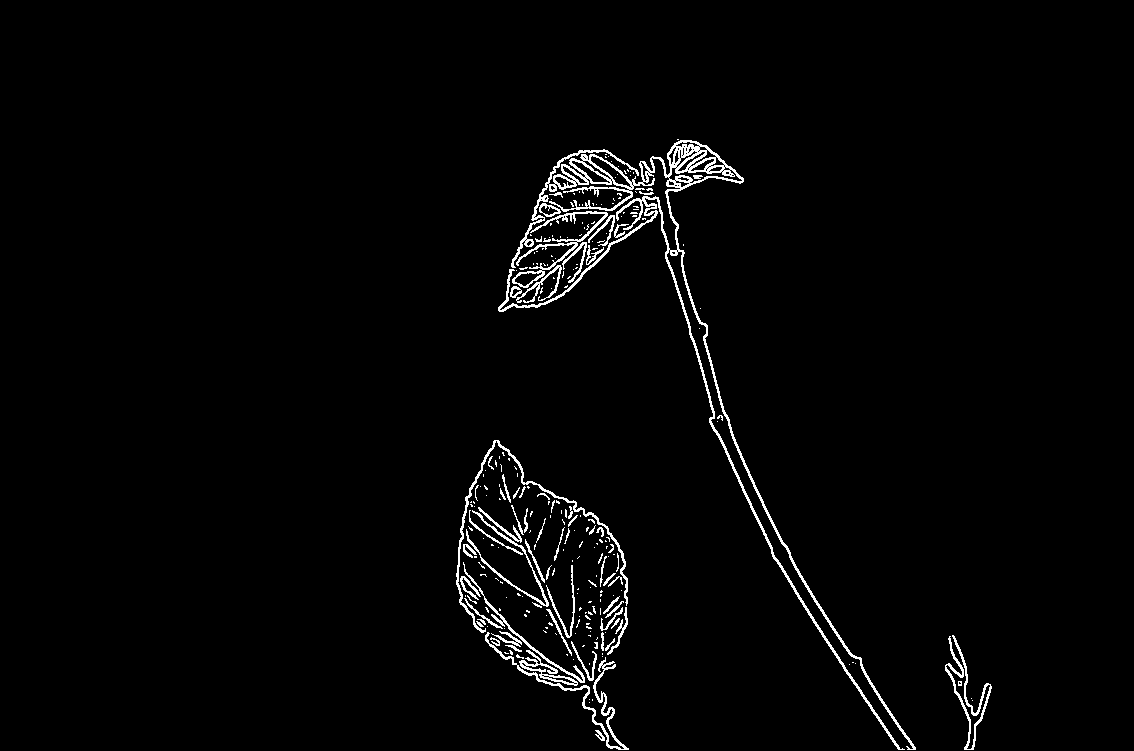
\includegraphics[width=7cm]{MH_alpha=0.2_leaf.png}
  \caption{MH处理后的($th=0.2$)}
  \end{minipage}
\end{figure}


\begin{figure}[H]
  \centering
  \begin{minipage}[t]{0.48\textwidth}
  \centering
  
\includegraphics[width=7cm]{ayu.jpg}
  \caption{原图}
  \end{minipage}
  \begin{minipage}[t]{0.48\textwidth}
  \centering
  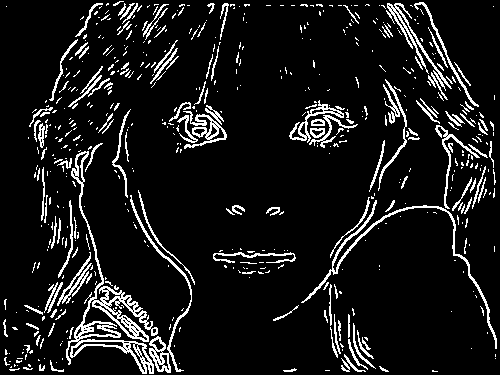
\includegraphics[width=7cm]{MH_alpha=0.15_ayu.png}
  \caption{MH处理后的($th=0.15$)}
  \end{minipage}
\end{figure}

\begin{figure}[H]
  \centering
  \begin{minipage}[t]{0.48\textwidth}
  \centering
  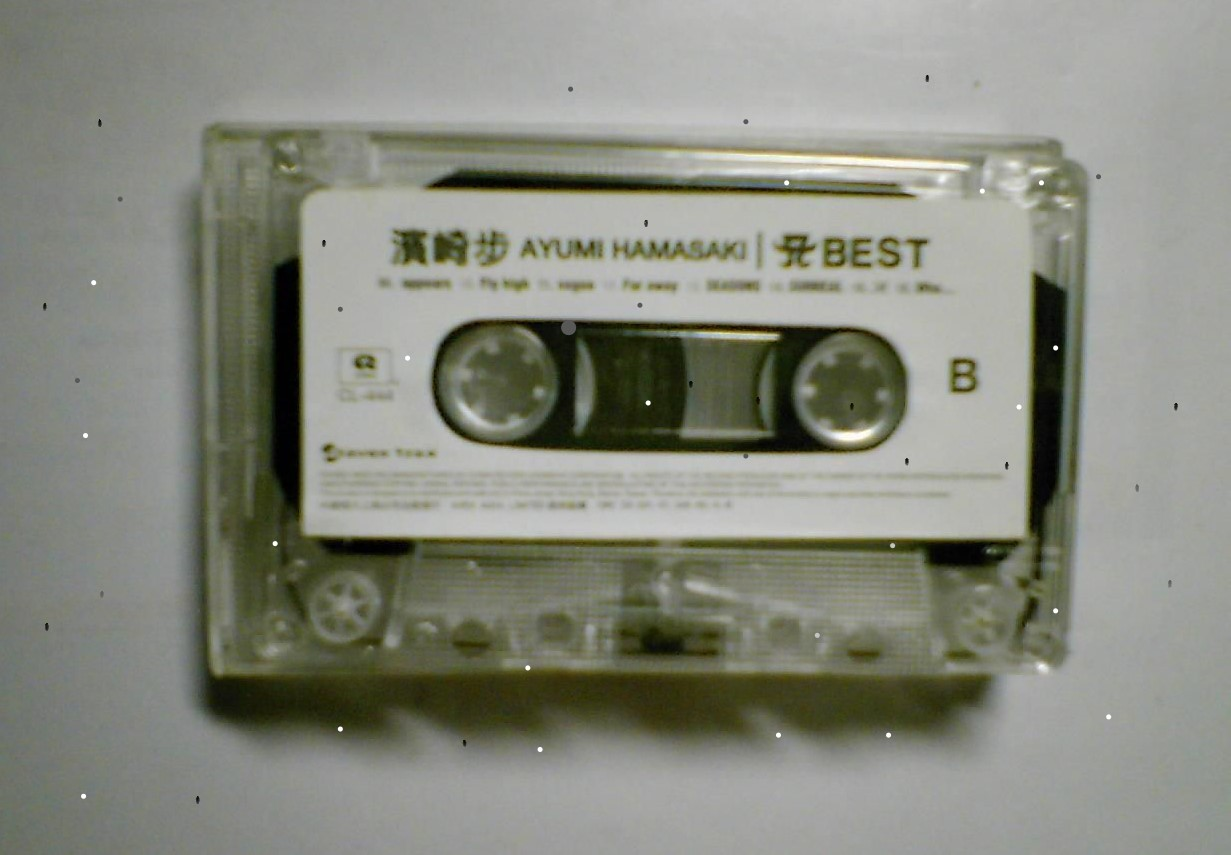
\includegraphics[width=7cm]{noise.jpg}
  \caption{原图}
  \end{minipage}
  \begin{minipage}[t]{0.48\textwidth}
  \centering
  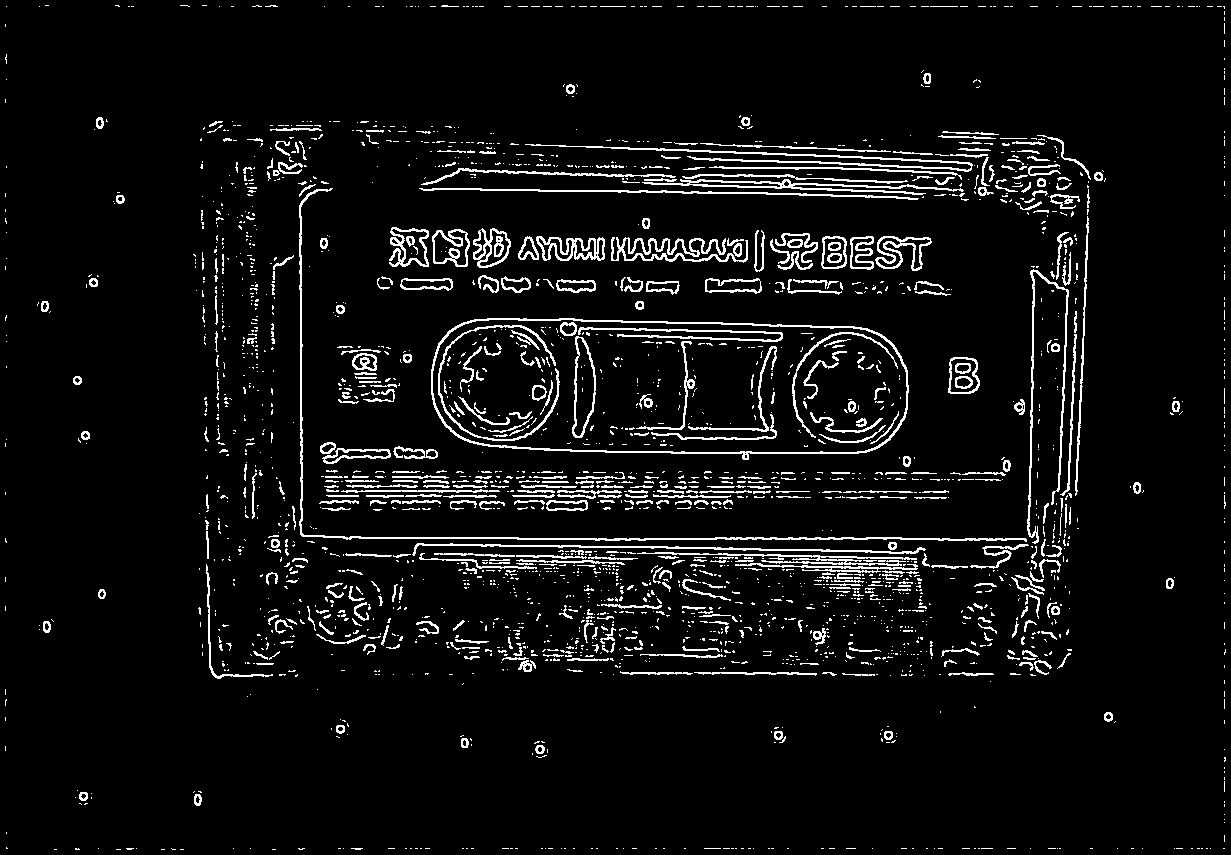
\includegraphics[width=7cm]{MH_alpha=0.055_noise.png}
  \caption{MH处理后的($th=0.055$)}
  \end{minipage}
\end{figure}





\subsection{Canny边缘检测器}
\subsubsection{实现原理}
Canny边缘检测器的实现在$Canny.m$文件中,实现方法与sobel算子类似,主要的过程是
\begin{enumerate}
  \item 用$n \times n$的高斯低通滤波器平滑图像$G$得到$G'$($n$是大于等于$6\sigma$的最小奇数)
  \item 计算$G'$的梯度大小$grad$和方向$alpha$,
  \item 非最大化抑制:我是对四个方向做非最大化抑制,如果该方向的邻居有比当前点大的抑制当前点 
  \item 滞后阈值和联通性分析:对于每一个大于$TH$的点,设置为1,再对它的八连通点进行分析,如果大于$TL$,则也设置为1.
\end{enumerate}
Canny边缘检测器需要设置的主要有两个参数:高阈值($TH$)和低阈值($TL$).

\subsubsection{实现效果}
\begin{figure}[H]
  \centering
  \begin{minipage}[t]{0.48\textwidth}
  \centering
  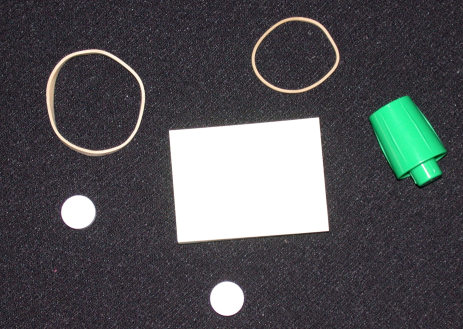
\includegraphics[width=7cm]{rubberband_cap.png}
  \caption{原图}
  \end{minipage}
  \begin{minipage}[t]{0.48\textwidth}
  \centering
  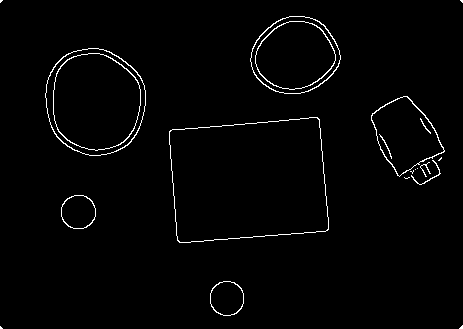
\includegraphics[width=7cm]{Canny_TH=0.02_TL=0.01_rubberband_cap.png}
  \caption{Canny处理后的($TH=0.02,TL=0.01$)}
  \end{minipage}
\end{figure}


\begin{figure}[H]
  \centering
  \begin{minipage}[t]{0.48\textwidth}
  \centering
  \includegraphics[width=7cm]{lena.png}
  \caption{原图}
  \end{minipage}
  \begin{minipage}[t]{0.48\textwidth}
  \centering
  \includegraphics[width=7cm]{Canny_TH=0.025_TL=0.01_lena.png}
  \caption{Canny处理后的($TH=0.025,TL=0.01$)}
  \end{minipage}
\end{figure}


\begin{figure}[H]
  \centering
  \begin{minipage}[t]{0.48\textwidth}
  \centering
  \includegraphics[width=7cm]{giraffe.jpg}
  \caption{原图}
  \end{minipage}
  \begin{minipage}[t]{0.48\textwidth}
  \centering
  \includegraphics[width=7cm]{Canny_TH=0.035_TL=0.015_giraffe.png}
  \caption{Canny处理后的($TH=0.035,TL=0.015$)}
  \end{minipage}
\end{figure}

\begin{figure}[H]
  \centering
  \begin{minipage}[t]{0.48\textwidth}
  \centering
  \includegraphics[width=7cm]{leaf.jpg}
  \caption{原图}
  \end{minipage}
  \begin{minipage}[t]{0.48\textwidth}
  \centering
  \includegraphics[width=7cm]{Canny_TH=0.015_TL=0.006_leaf.png}
  \caption{Canny处理后的($TH=0.015,TL=0.006$)}
  \end{minipage}
\end{figure}


\begin{figure}[H]
  \centering
  \begin{minipage}[t]{0.48\textwidth}
  \centering
  \includegraphics[width=7cm]{ayu.jpg}
  \caption{原图}
  \end{minipage}
  \begin{minipage}[t]{0.48\textwidth}
  \centering
  \includegraphics[width=7cm]{Canny_TH=0.02_TL=0.01_ayu.png}
  \caption{Canny处理后的($TH=0.02,TL=0.01$)}
  \end{minipage}
\end{figure}

\begin{figure}[H]
  \centering
  \begin{minipage}[t]{0.48\textwidth}
  \centering
  \includegraphics[width=7cm]{noise.jpg}
  \caption{原图}
  \end{minipage}
  \begin{minipage}[t]{0.48\textwidth}
  \centering
  \includegraphics[width=7cm]{Canny_TH=0.015_TL=0.005_noise.png}
  \caption{Canny处理后的($TH=0.015,TL=0.005$)}
  \end{minipage}
\end{figure}


\subsection{Marr-Hildreth和Canny边缘检测器总结}
在MH中,阈值比例$th$的选取对结果的影响是比较大的。同样的,在Canny中,低阈值$TL$和高阈值$TH$的选取对结果的影响也是比较大的。

因为有非最大抑制,所以Canny的边缘较细。而MH的边缘较粗,但比sobel算子和prewitt算子的细。


Canny在边缘不间断上做的要比MH好。如下面两张图的对比:

\begin{figure}[H]
  \centering
  \begin{minipage}[t]{0.48\textwidth}
    \centering
    \includegraphics[width=7cm]{MH_alpha=0.35_rubberband_cap.png}
    \caption{MH处理后的($th=0.35$)}
    \end{minipage}
  \begin{minipage}[t]{0.48\textwidth}
  \centering
  \includegraphics[width=7cm]{Canny_TH=0.02_TL=0.01_rubberband_cap.png}
  \caption{Canny处理后的($TH=0.02,TL=0.01$)}
  \end{minipage}
\end{figure}



\section{边缘连接}



对于边缘连接,我使用Moore-Neighbor Tracing算法。用imtool来定界,确定一个点后,使用该算法就能得出一个轮廓。

\subsection{Moore-Neighbor Tracing}

\subsubsection{实现原理}
Moore-Neighbor Tracing算法的实现主要在$my\_edgelinking.m$中,主要的算法流程是:
  \begin{enumerate}
    \item 设输入图像为$G$, 输入的起始点为$s(row,col)$
    \item 设$c$为$N(s)$顺时针方向中的一个点。($N(s)$表示$s$的邻域集合)
    \item 将$s$加入到$B$中
    \item 当不满足终止条件时,反复执行下列步骤,否则返回B
    \item 如果$G(c)=1$,那么
      \begin{itemize}
        \item 令$p=c$
        \item 将$c$加入$B$中
        \item 更新方向向量
      \end{itemize}
    \item 方向向量递增,选择$N(p)$中相应方向的点。
  \end{enumerate}

终止条件可以设置为到达$s$多次,或者以相同的方向进入$s$.


\subsubsection{实现效果}

\begin{figure}[H]
  \centering
  \begin{minipage}[t]{0.48\textwidth}
  \centering
  \includegraphics[width=7cm]{Canny_TH=0.02_TL=0.01_rubberband_cap.png}
  \caption{Canny处理后}
  \end{minipage}
  \begin{minipage}[t]{0.48\textwidth}
  \centering
  \includegraphics[width=7cm]{contour_full.png}
  \caption{进一步边缘连接后}
  \end{minipage}
\end{figure}



\end{document}